\documentclass[aspectratio=169,11pt]{beamer}

\usetheme{Madrid}
\setbeamertemplate{navigation symbols}{}

\usepackage{amsmath,amssymb}
\usepackage{graphicx}
\usepackage{currfile}

\title[PBC and PS Artifact]{PBC, Power Spectrum, and the Square Artifact}
\author{Alexandros Tsouros}
\date{}

\graphicspath{{\currfiledir}{\currfiledir figures/}{figures/}}

\begin{document}

\begin{frame}[fragile]
  \titlepage
\end{frame}

\begin{frame}[fragile]{Full 5-channel object}
In the full phase, the power-spectrum loss is computed from the same
5-channel object as the scattering loss:
\[
  X^{(i)}
  =
  \begin{bmatrix}
    d_Q\\
    n_Q^{(i)}\\
    d_U\\
    n_U^{(i)}\\
    d_I
  \end{bmatrix}
  \quad\text{or}\quad
  X_{\mathrm{run}}^{(i)}(u)
  =
  \begin{bmatrix}
    u_Q+n_Q^{(i)}\\
    d_Q-u_Q\\
    u_U+n_U^{(i)}\\
    d_U-u_U\\
    d_I
  \end{bmatrix}.
\]

\vspace{0.25em}
For a minibatch,
\[
  X\in\mathbb{R}^{N_b\times5\times N\times N}.
\]
\end{frame}

\begin{frame}[fragile]{What the PS term measures}
For each radial Fourier bin $b$, the code builds a mask $M_b(k)$ and estimates
channel-pair spectra:
\[
  P(X)\in\mathbb{C}^{N_b\times5\times5\times B}.
\]

\vspace{0.25em}
The two channel indices mean that each coefficient compares a pair
$(c_1,c_2)$:
\[
  P_{c_1c_2b}
  \sim
  \left\langle
    M_b(k)\widehat X_{c_1}(k)
    \overline{\widehat X_{c_2}(k)}
  \right\rangle.
\]

\vspace{0.25em}
The issue was not the existence of this constraint, but how the non-periodic
branch estimated it.
\end{frame}

\begin{frame}[fragile]{When \texttt{PBC=True}}
With \texttt{PBC=True}, the map is treated as periodic and the PS computation
stays in Fourier space:
\[
  P^{\mathrm{pbc}}_{a,c_1,c_2,b}
  =
  \frac{
    \sum_k
    M_b(k)\widehat X_{a,c_1}(k)
    \overline{\widehat X_{a,c_2}(k)}
  }{
    \sum_k M_b(k)
  }.
\]

\vspace{0.25em}
There is no real-space crop mask in this branch.

\vspace{0.25em}
So the PS gradient is spatially uniform with respect to the image support:
it does not introduce an explicit square window in real space.
\end{frame}

\begin{frame}[fragile]{When \texttt{PBC=False}}
With \texttt{PBC=False}, the code tries to avoid edge contamination from the
FFT by moving back to real space after binning:
\[
  X^{(b)}_{a,c}(x)
  =
  \mathcal{F}^{-1}
  \left[
    M_b(k)\widehat X_{a,c}(k)
  \right](x).
\]

\vspace{0.25em}
Then it computes the channel-pair product only on a retained central region:
\[
  P^{\mathrm{nonpbc}}_{a,c_1,c_2,b}
  \propto
  \sum_x
  W_b(x)
  X^{(b)}_{a,c_1}(x)
  \overline{X_{a,c_2}(x)}.
\]

\vspace{0.25em}
Originally,
\[
  W_b(x)\in\{0,1\}
\]
was a hard, bin-dependent square crop mask.
\end{frame}

\begin{frame}[fragile]{Why this made a square artifact}
The hard mask created a sharp real-space boundary:
\[
  W_b(x)
  =
  \begin{cases}
    1, & x \text{ inside the central square},\\
    0, & x \text{ near the boundary}.
  \end{cases}
\]

\vspace{0.25em}
When the PS loss is backpropagated, the recovered maps $u_Q,u_U$ receive
gradients through this square weighting.

\vspace{0.25em}
So the optimizer was not only matching radial Fourier power. In the
\texttt{PBC=False} PS branch, it was also seeing a bin-dependent square support.

\vspace{0.25em}
This seems to explain why the artifact appeared for
\[
  \texttt{PBC=False},\quad \texttt{ST\_COMPUTE\_PS=True},
\]
but not for \texttt{PBC=True}.
\end{frame}

\begin{frame}[fragile]{Before change: map}
\centering
\IfFileExists{figures/PBC=False, ST_COMPUTE_PS=True_maps.png}{%
  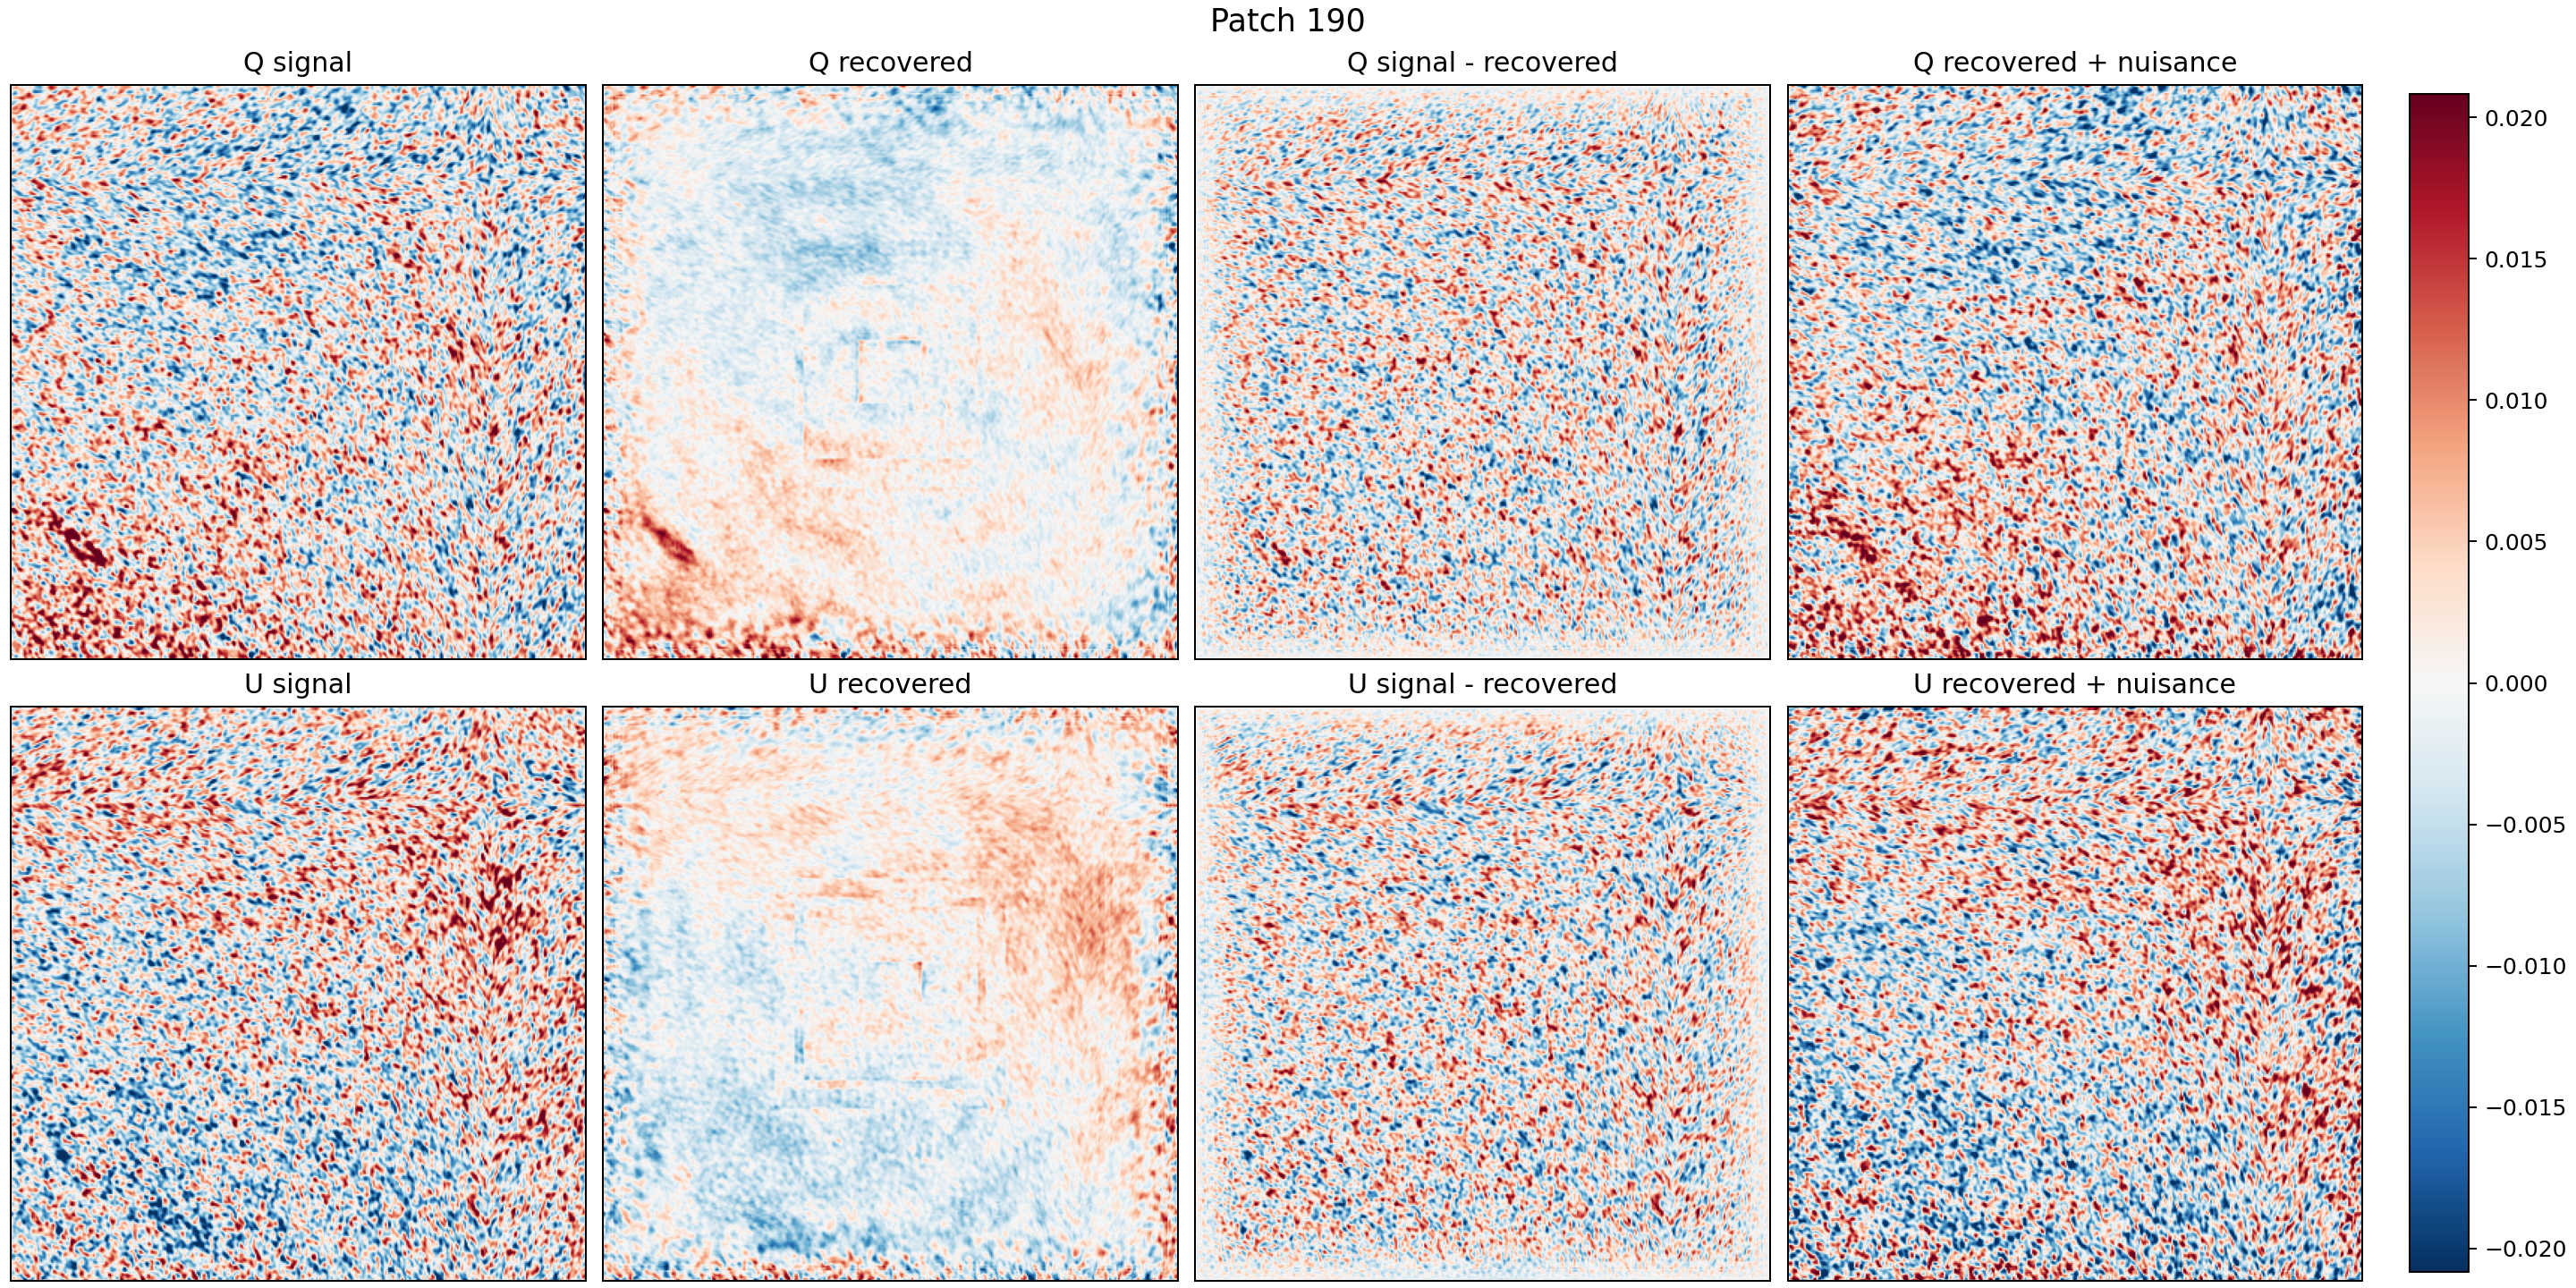
\includegraphics[width=\textwidth,height=0.82\textheight,keepaspectratio]{figures/PBC=False, ST_COMPUTE_PS=True_maps.png}
}{%
  \vspace{2em}
  \texttt{figures/PBC=False, ST\_COMPUTE\_PS=True\_maps.png}
}

\vspace{0.25em}
\texttt{PBC=False}, \texttt{ST\_COMPUTE\_PS=True}: hard square crop mask.
\end{frame}

\begin{frame}[fragile]{Periodic comparison: map}
\centering
\IfFileExists{figures/PBC=True, ST_COMPUTE_PS=True_maps.png}{%
  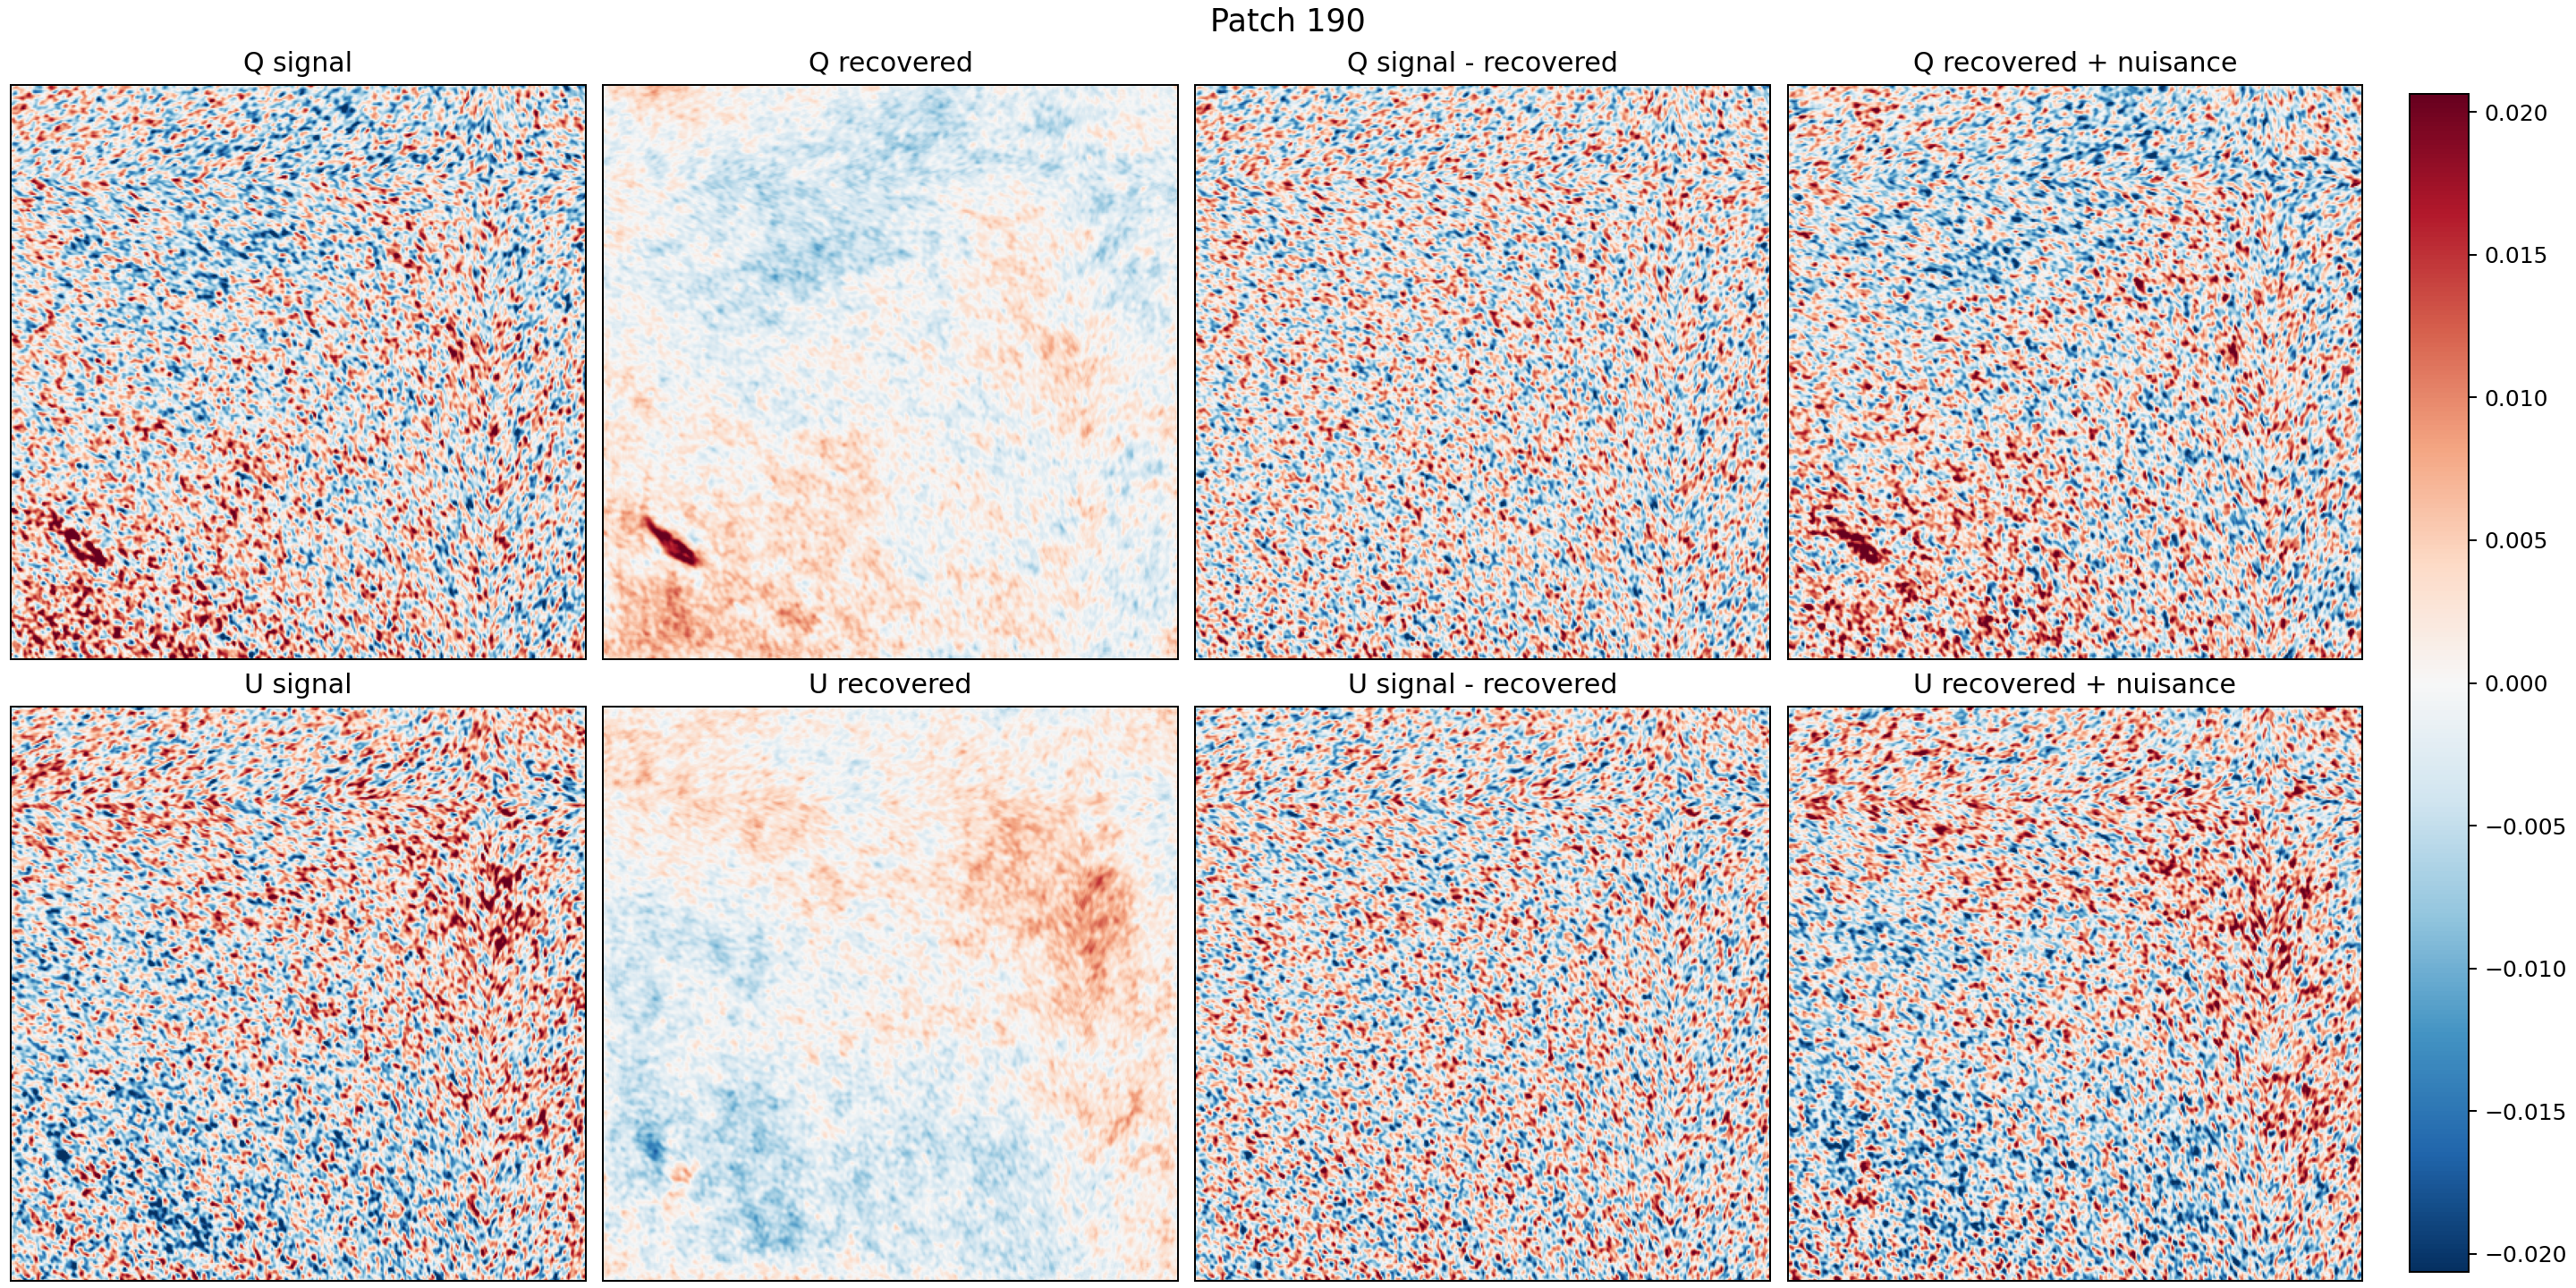
\includegraphics[width=\textwidth,height=0.82\textheight,keepaspectratio]{figures/PBC=True, ST_COMPUTE_PS=True_maps.png}
}{%
  \vspace{2em}
  \texttt{figures/PBC=True, ST\_COMPUTE\_PS=True\_maps.png}
}

\vspace{0.25em}
\texttt{PBC=True}, \texttt{ST\_COMPUTE\_PS=True}: no real-space crop mask.
\end{frame}

\begin{frame}[fragile]{After change: map}
\centering
\IfFileExists{figures/p190_m384_fft_f64_s2_r0_i0_p0_n0_bumpsteerable_2a61a1a2e1_maps.png}{%
  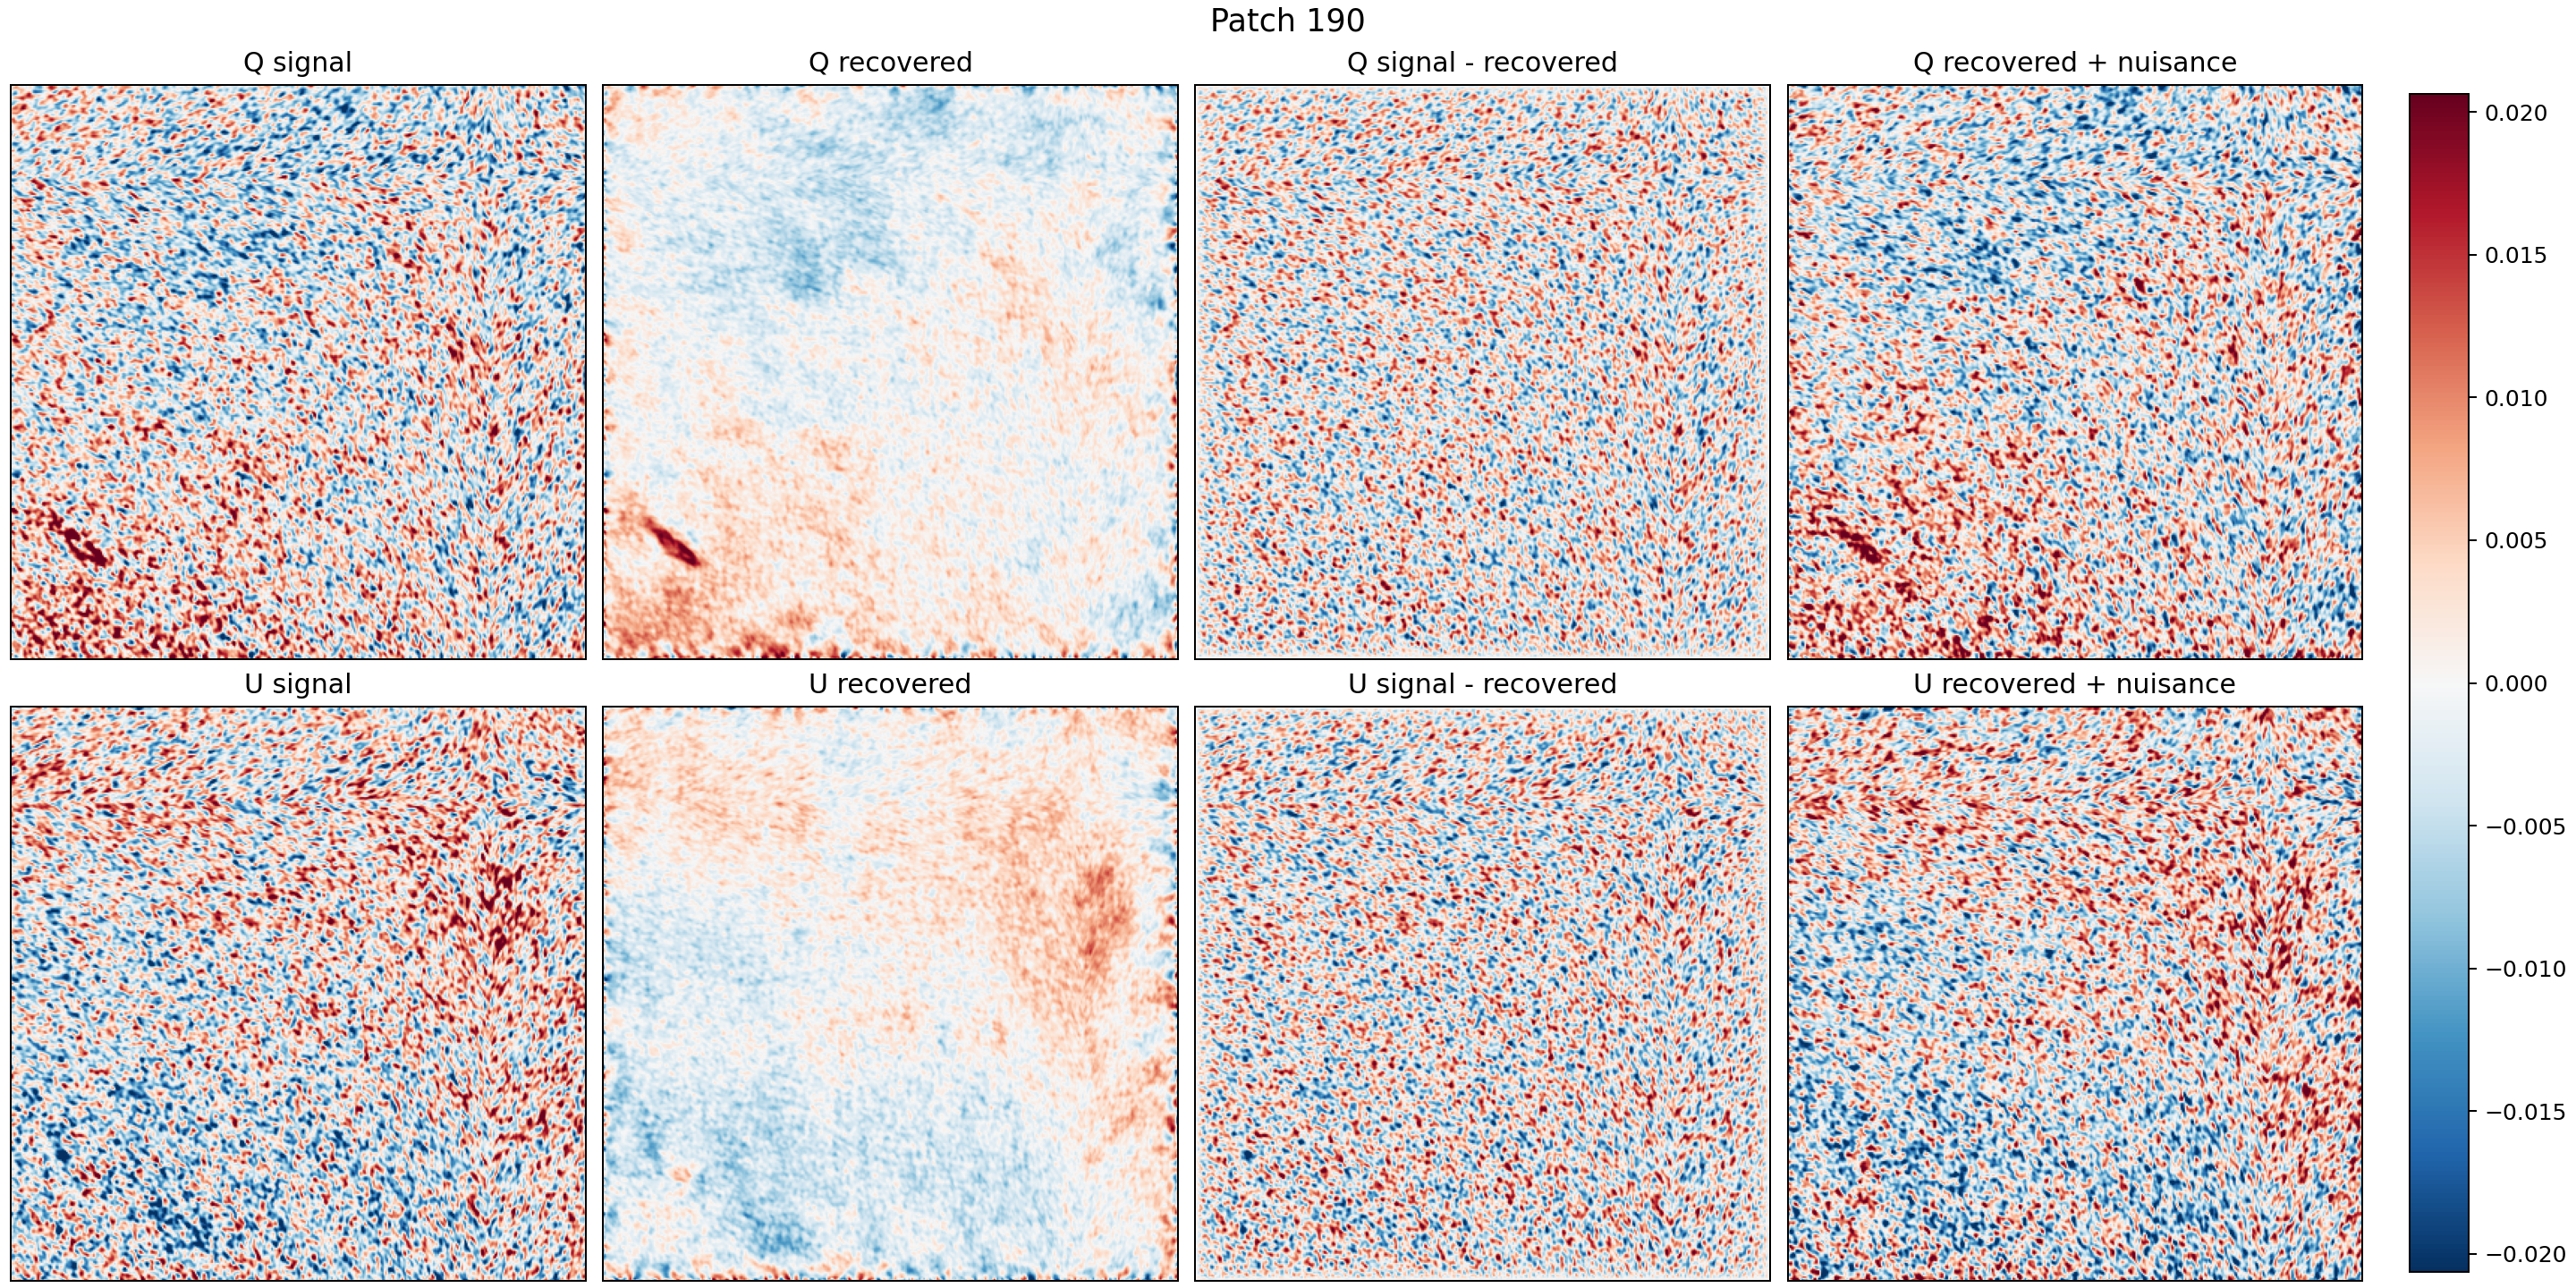
\includegraphics[width=\textwidth,height=0.82\textheight,keepaspectratio]{figures/p190_m384_fft_f64_s2_r0_i0_p0_n0_bumpsteerable_2a61a1a2e1_maps.png}
}{%
  \vspace{2em}
  \texttt{figures/p190\_m384\_...\_2a61a1a2e1\_maps.png}
}

\vspace{0.25em}
\texttt{PBC=False}, \texttt{ST\_COMPUTE\_PS=False}
\end{frame}

\begin{frame}[fragile]{After change: Q power spectrum}
\centering
\IfFileExists{figures/p190_m384_fft_f64_s2_r0_i0_p0_n0_bumpsteerable_2a61a1a2e1_power_spectrum_Q.png}{%
  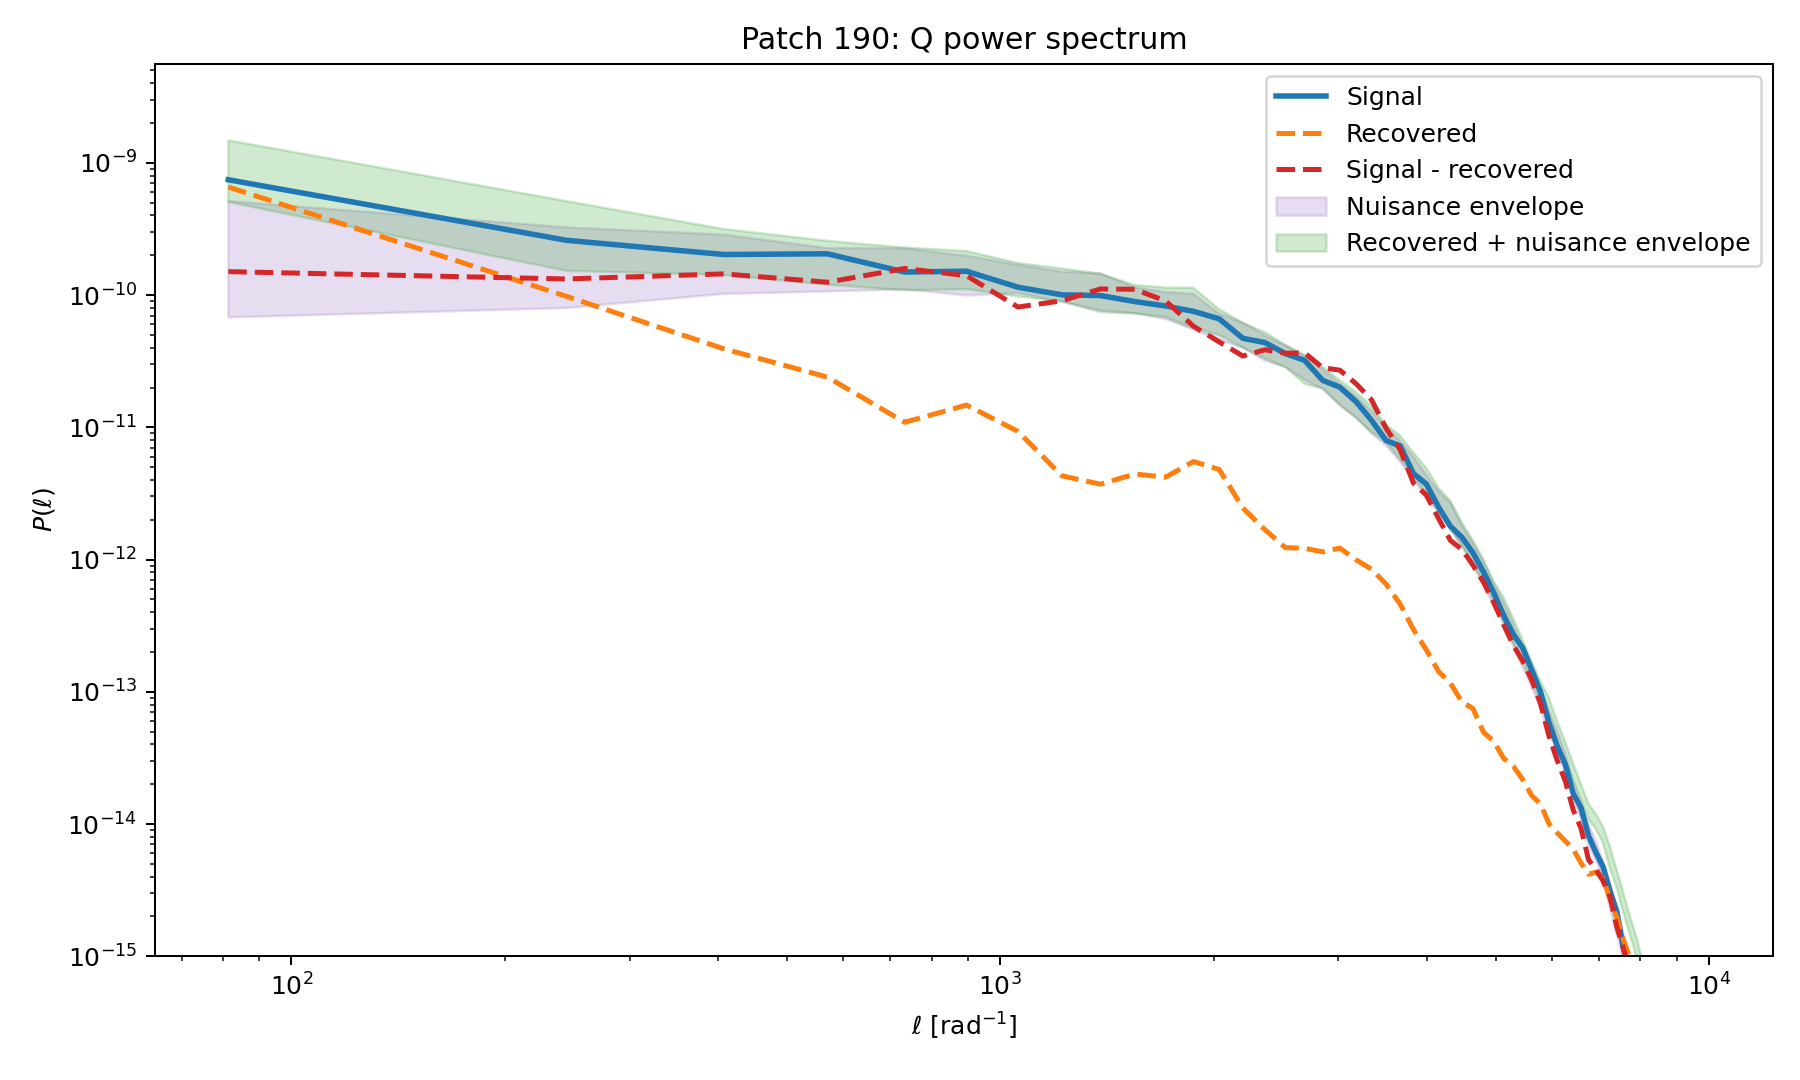
\includegraphics[width=\textwidth,height=0.82\textheight,keepaspectratio]{figures/p190_m384_fft_f64_s2_r0_i0_p0_n0_bumpsteerable_2a61a1a2e1_power_spectrum_Q.png}
}{%
  \vspace{2em}
  \texttt{figures/p190\_m384\_...\_2a61a1a2e1\_power\_spectrum\_Q.png}
}

\vspace{0.25em}
\texttt{PBC=False}, \texttt{ST\_COMPUTE\_PS=False}
\end{frame}

\begin{frame}[fragile]{After change: U power spectrum}
\centering
\IfFileExists{figures/p190_m384_fft_f64_s2_r0_i0_p0_n0_bumpsteerable_2a61a1a2e1_power_spectrum_U.png}{%
  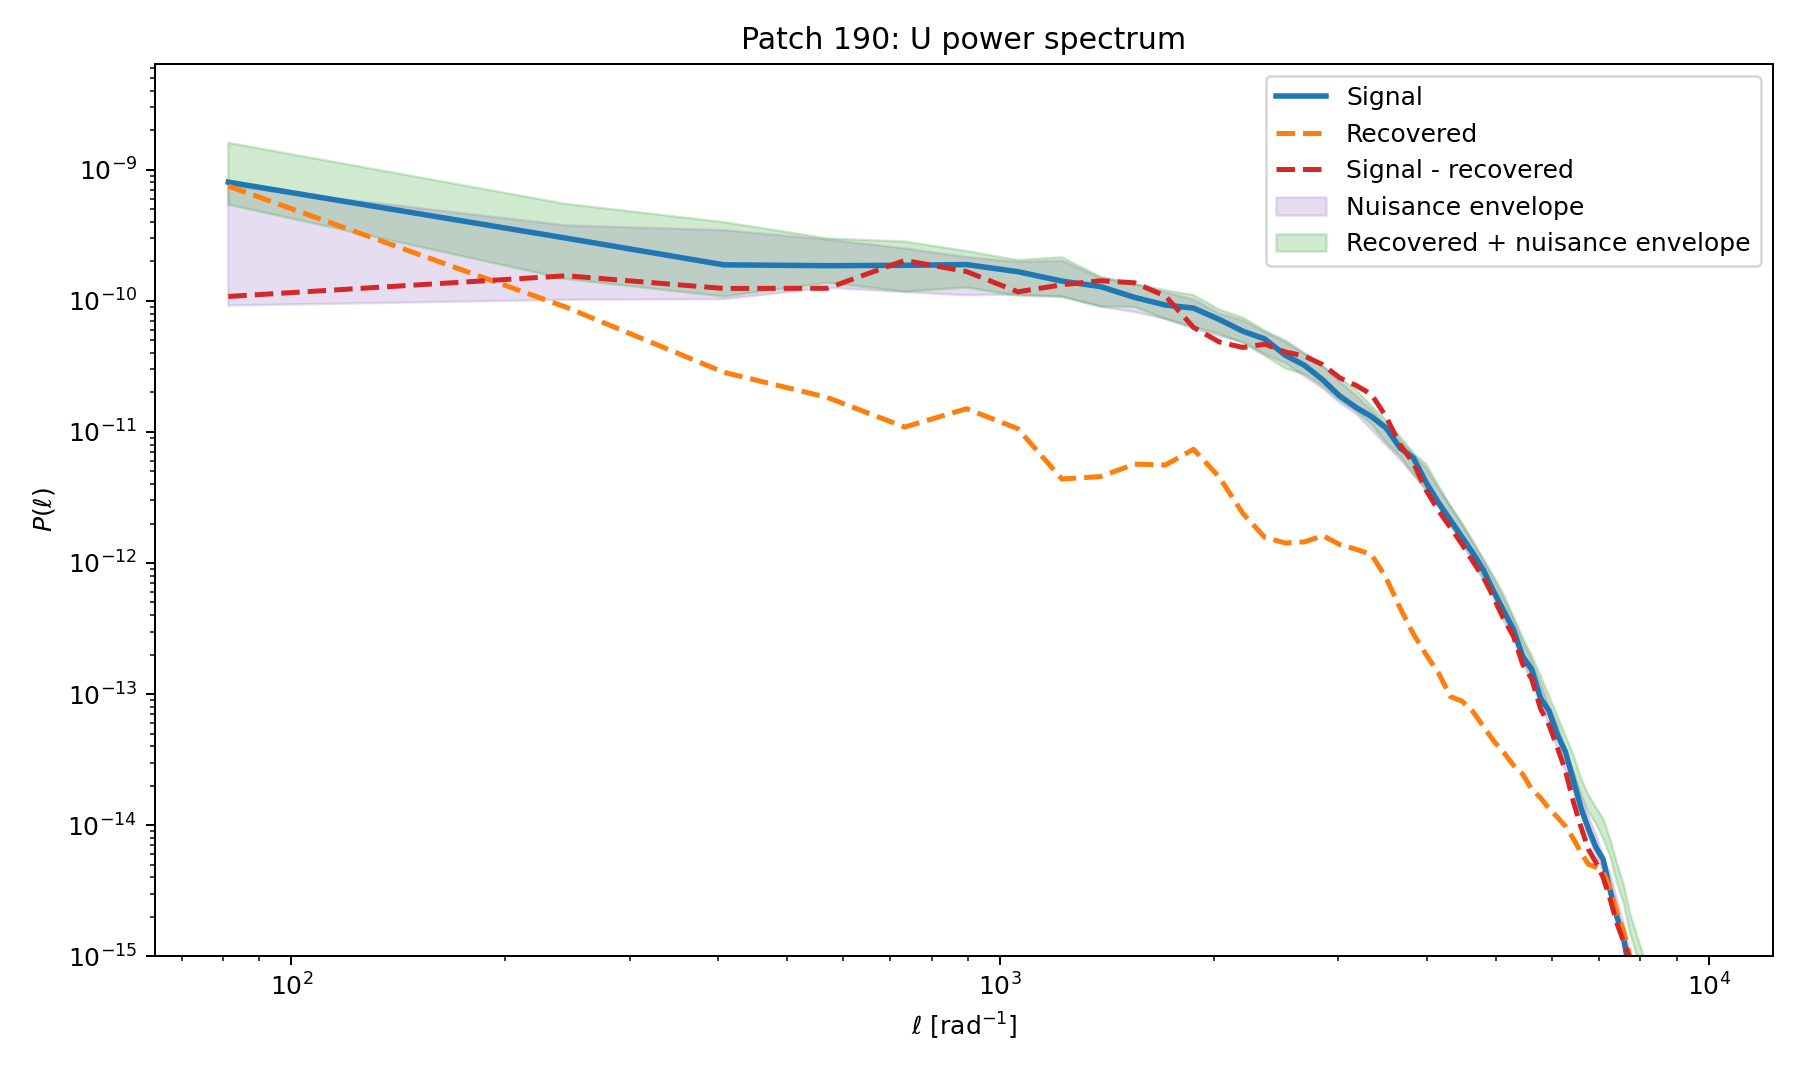
\includegraphics[width=\textwidth,height=0.82\textheight,keepaspectratio]{figures/p190_m384_fft_f64_s2_r0_i0_p0_n0_bumpsteerable_2a61a1a2e1_power_spectrum_U.png}
}{%
  \vspace{2em}
  \texttt{figures/p190\_m384\_...\_2a61a1a2e1\_power\_spectrum\_U.png}
}

\vspace{0.25em}
\texttt{PBC=False}, \texttt{ST\_COMPUTE\_PS=False}
\end{frame}

\begin{frame}[fragile]{No PS constraint: map}
\centering
\IfFileExists{figures/p190_m384_fft_f64_s2_r0_i0_p0_n0_bumpsteerable_e0163afa2f_maps.png}{%
  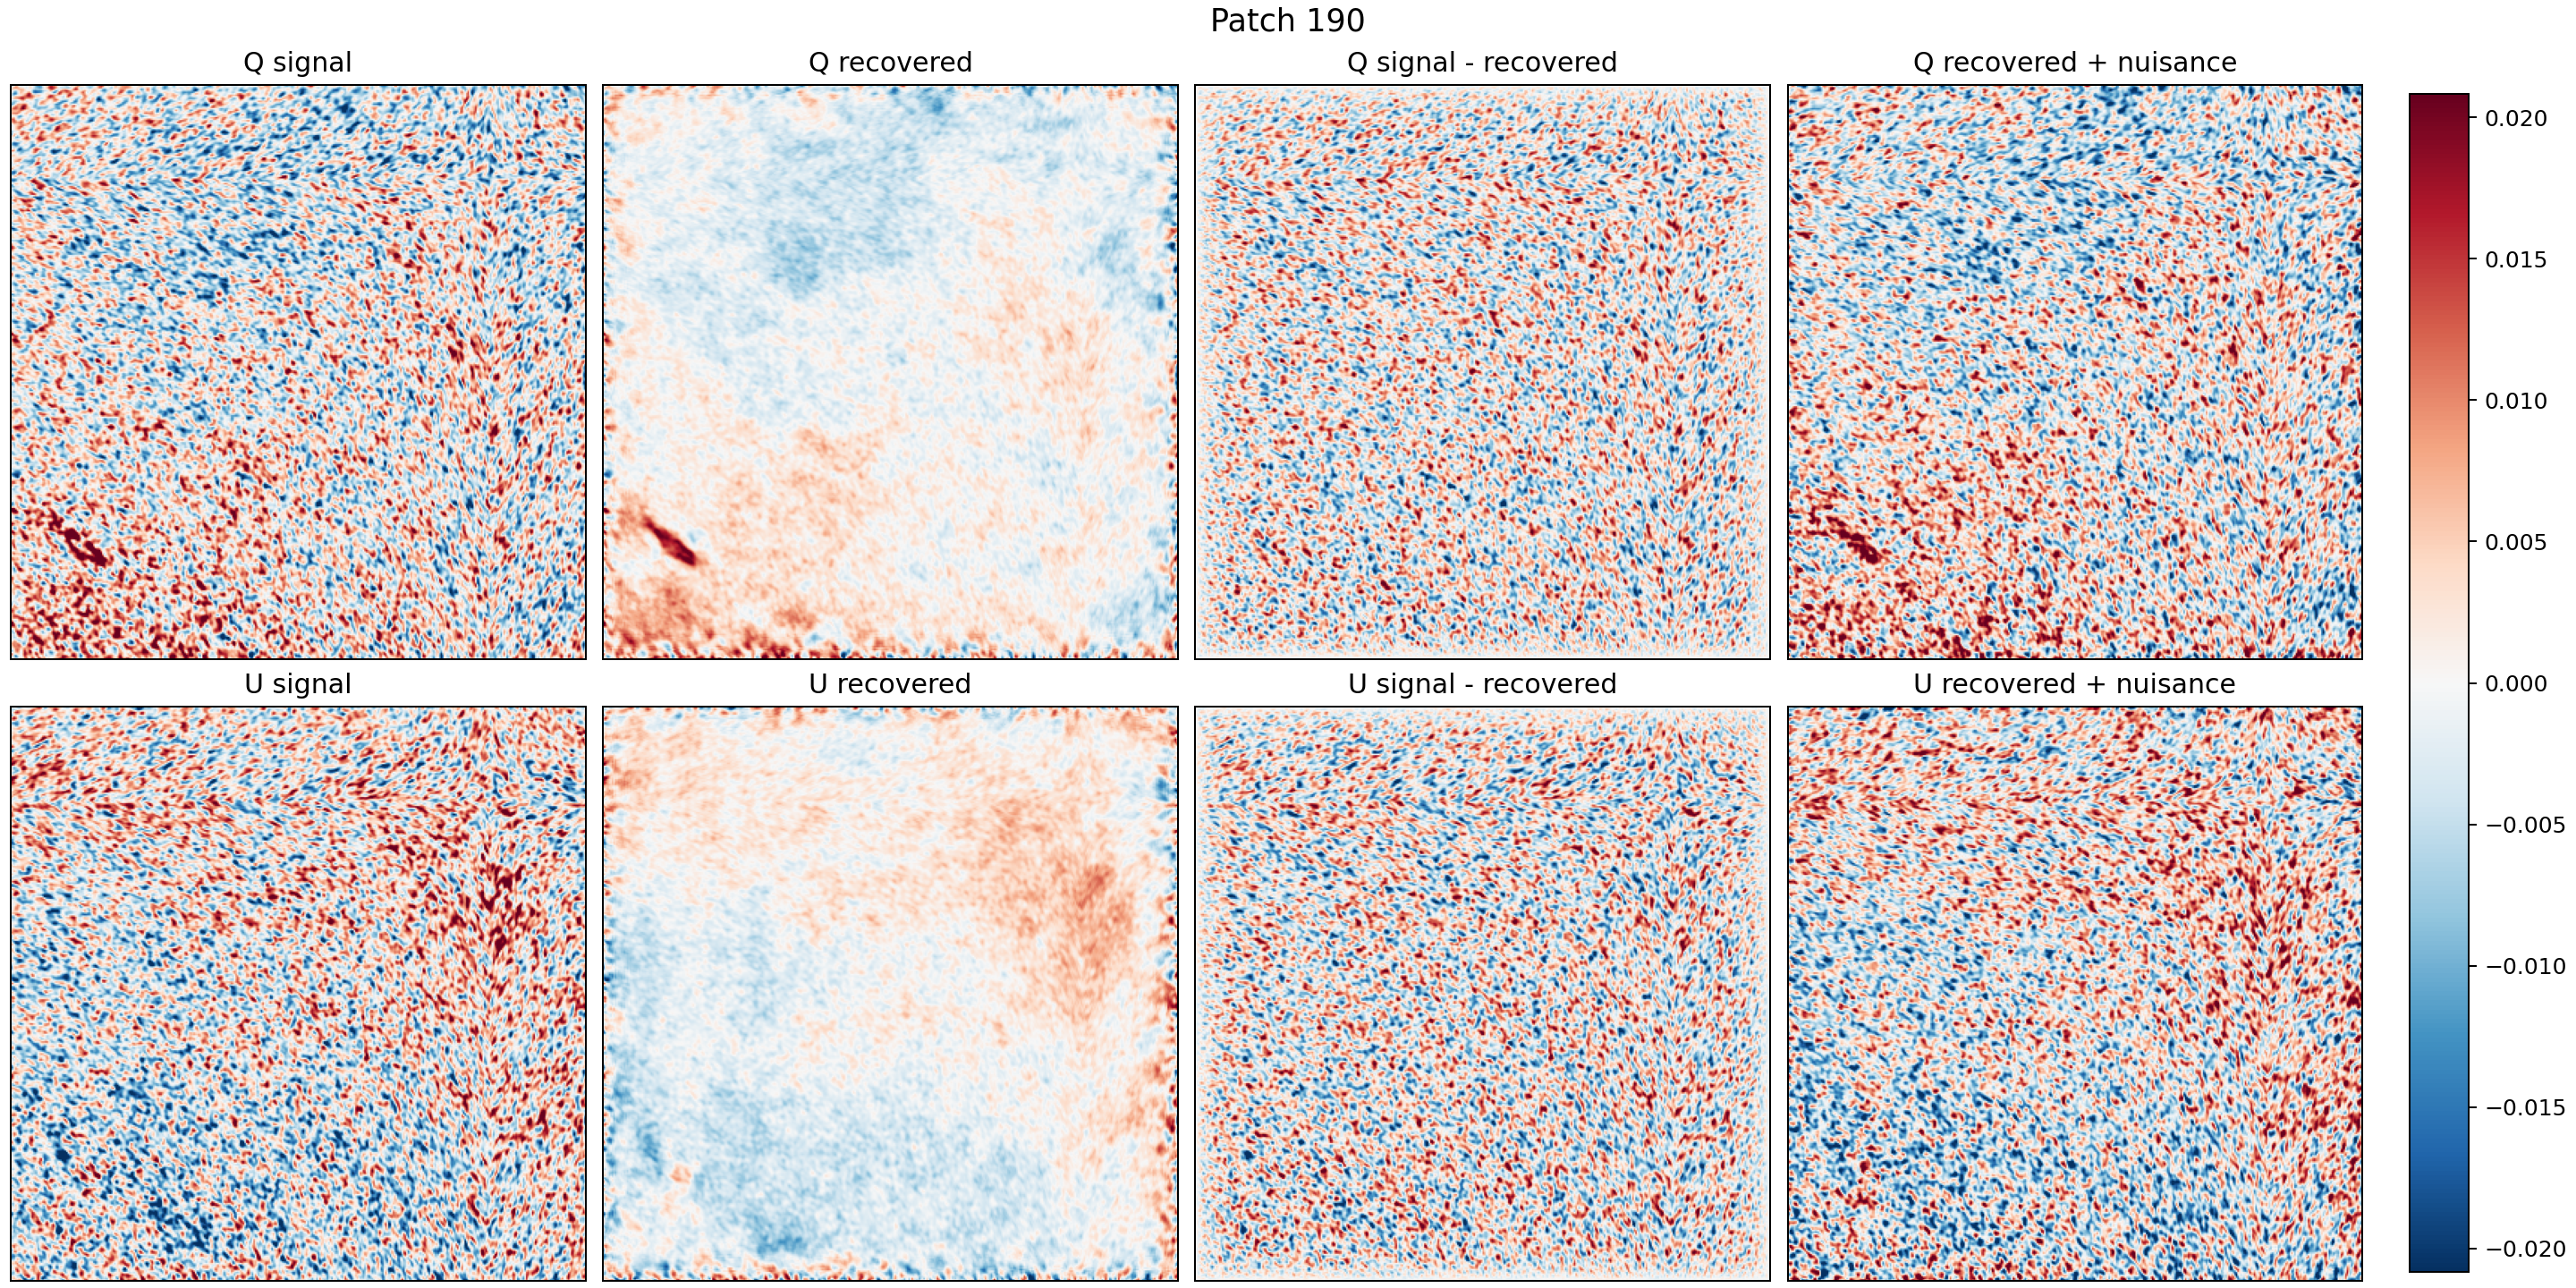
\includegraphics[width=\textwidth,height=0.82\textheight,keepaspectratio]{figures/p190_m384_fft_f64_s2_r0_i0_p0_n0_bumpsteerable_e0163afa2f_maps.png}
}{%
  \vspace{2em}
  \texttt{figures/p190\_m384\_...\_e0163afa2f\_maps.png}
}

\vspace{0.25em}
\texttt{PBC=False}, \texttt{ST\_COMPUTE\_PS=True}: smooth apodization mask
\end{frame}

\begin{frame}[fragile]{Q power spectrum}
\centering
\IfFileExists{figures/p190_m384_fft_f64_s2_r0_i0_p0_n0_bumpsteerable_e0163afa2f_power_spectrum_Q.png}{%
  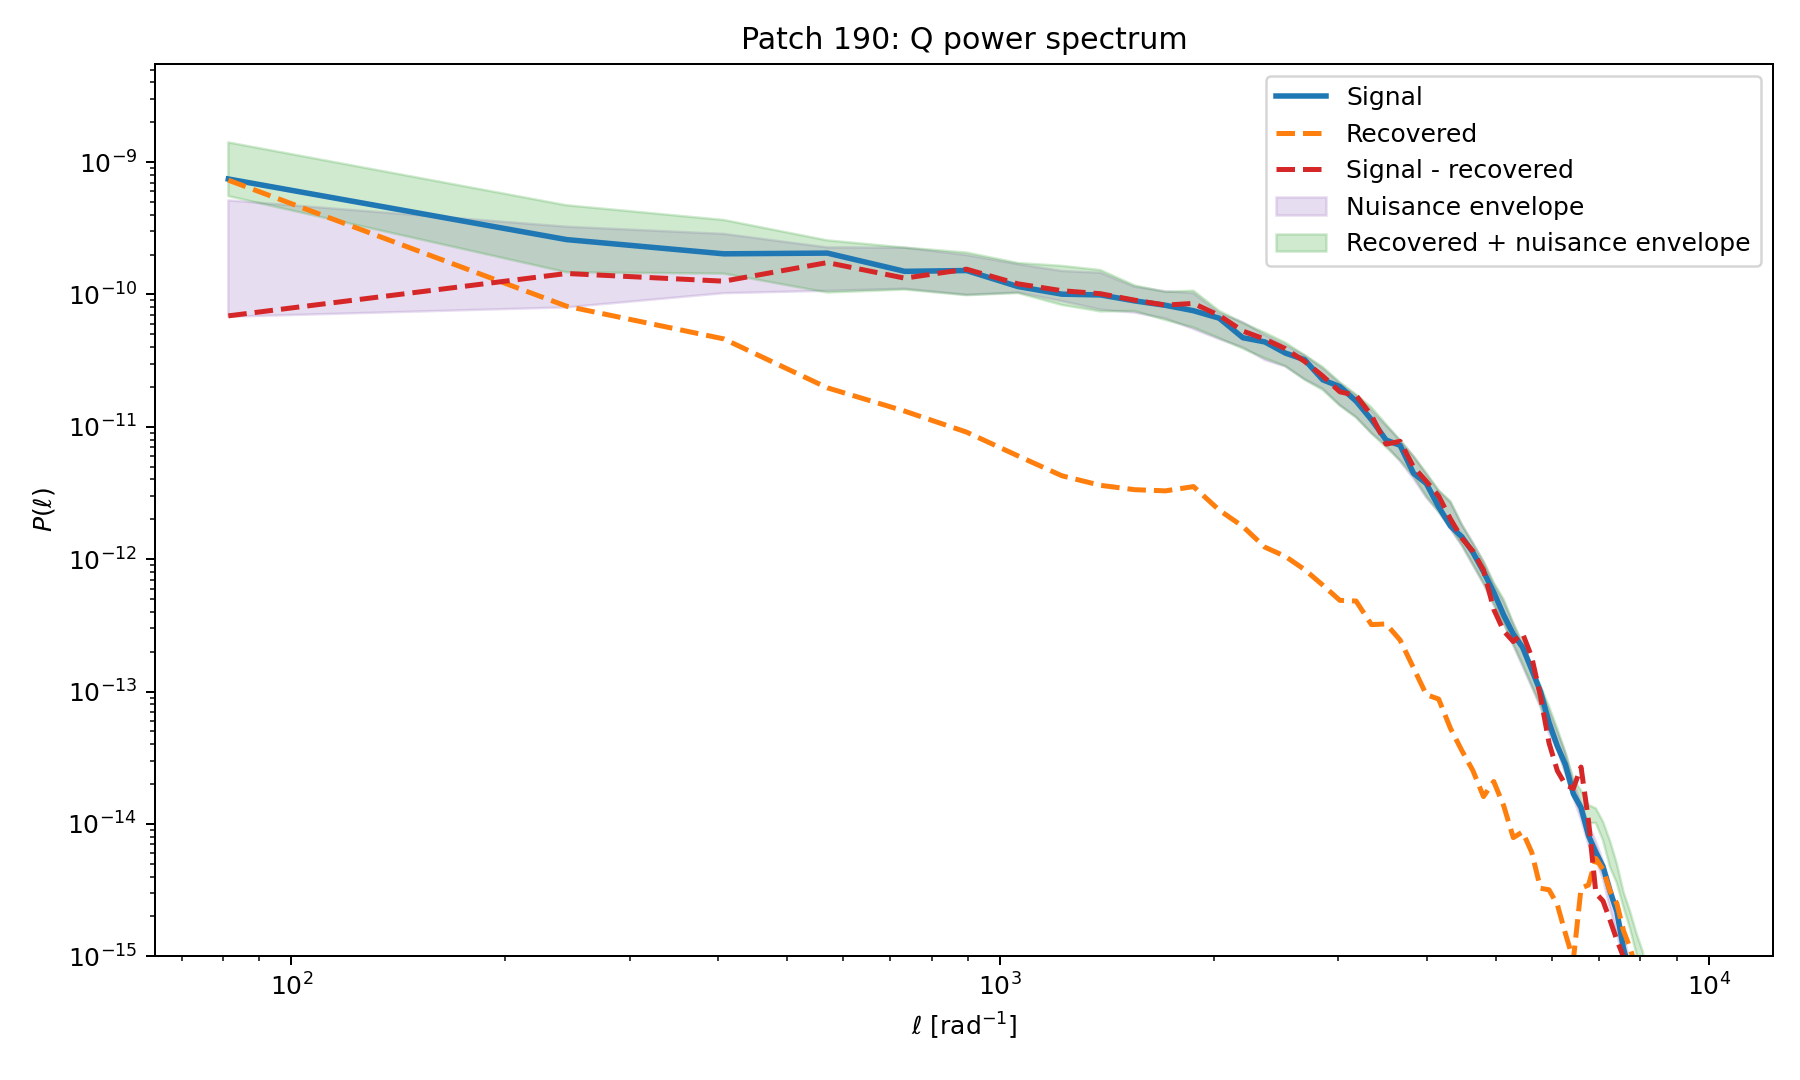
\includegraphics[width=\textwidth,height=0.82\textheight,keepaspectratio]{figures/p190_m384_fft_f64_s2_r0_i0_p0_n0_bumpsteerable_e0163afa2f_power_spectrum_Q.png}
}{%
  \vspace{2em}
  \texttt{figures/p190\_m384\_...\_e0163afa2f\_power\_spectrum\_Q.png}
}

\vspace{0.25em}
\texttt{PBC=False}, \texttt{ST\_COMPUTE\_PS=True}: smooth apodization mask
\end{frame}

\begin{frame}[fragile]{U power spectrum}
\centering
\IfFileExists{figures/p190_m384_fft_f64_s2_r0_i0_p0_n0_bumpsteerable_e0163afa2f_power_spectrum_U.png}{%
  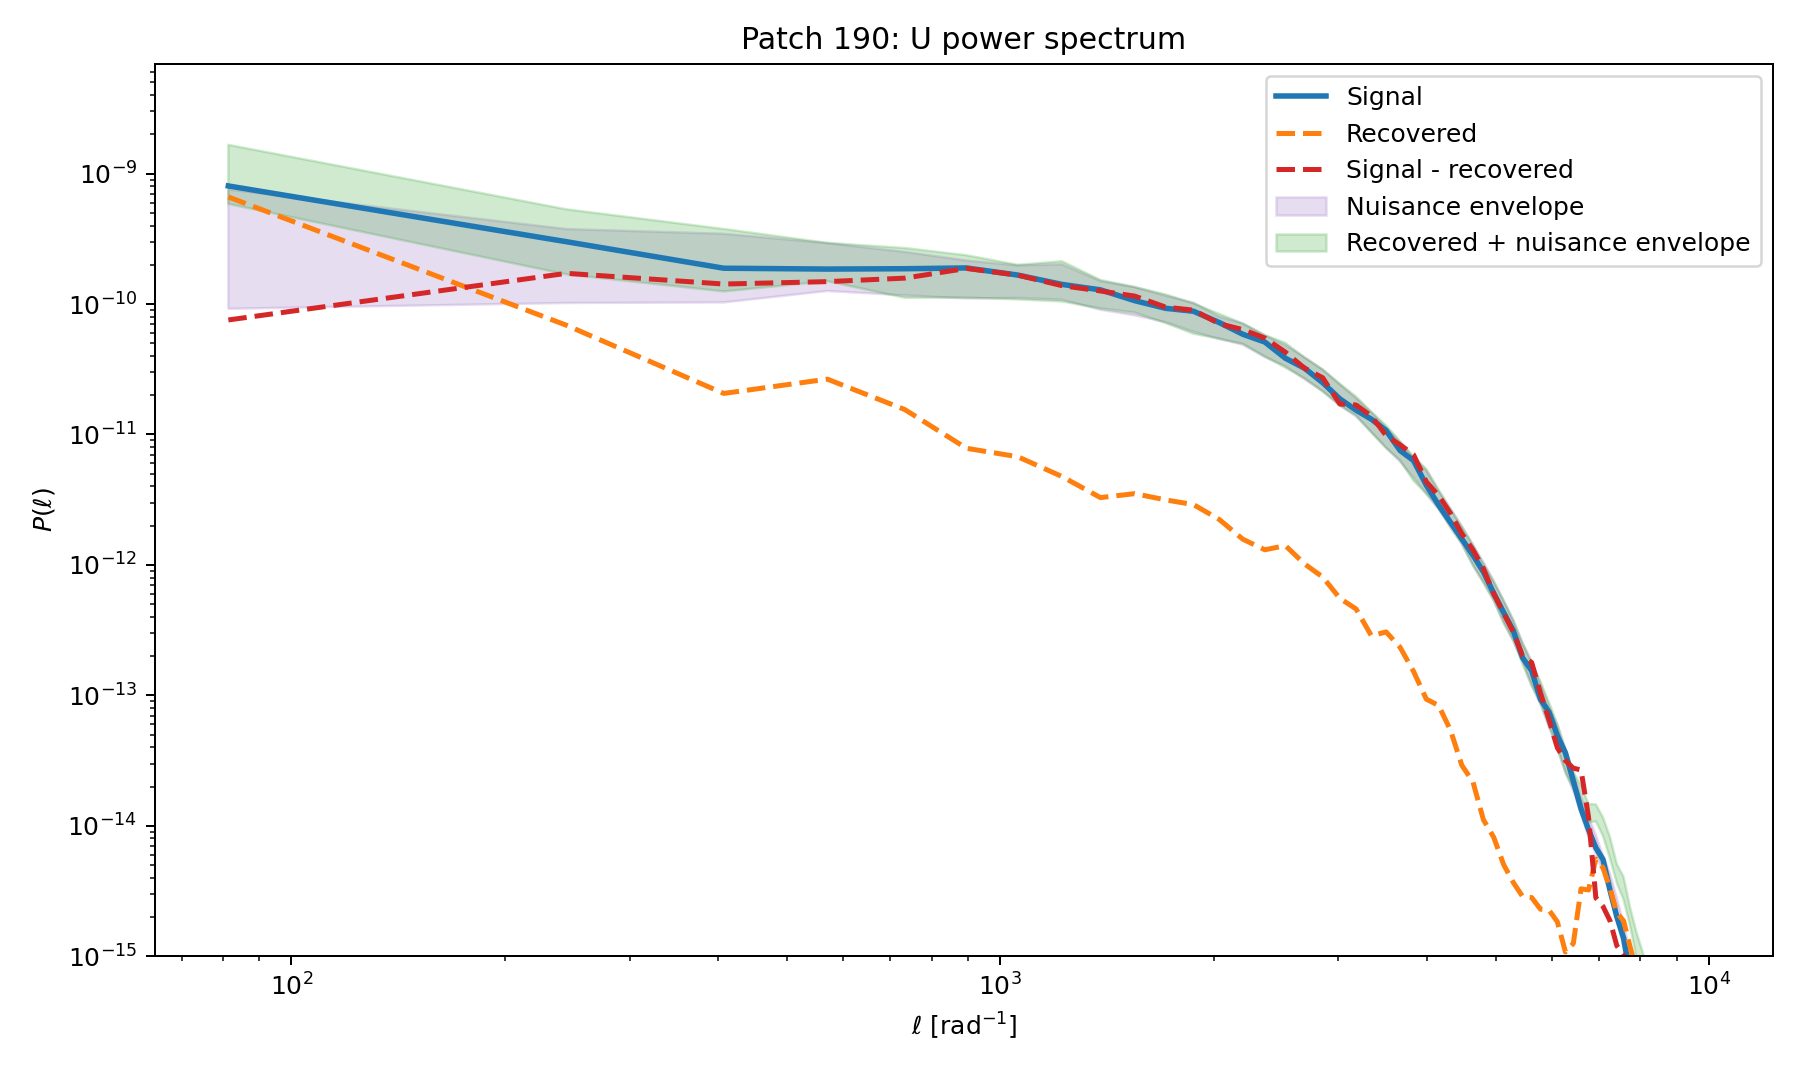
\includegraphics[width=\textwidth,height=0.82\textheight,keepaspectratio]{figures/p190_m384_fft_f64_s2_r0_i0_p0_n0_bumpsteerable_e0163afa2f_power_spectrum_U.png}
}{%
  \vspace{2em}
  \texttt{figures/p190\_m384\_...\_e0163afa2f\_power\_spectrum\_U.png}
}

\vspace{0.25em}
\texttt{PBC=False}, \texttt{ST\_COMPUTE\_PS=True}: smooth apodization mask
\end{frame}

\begin{frame}[fragile]{Update pixel space mask}
The change was made only in the non-periodic PS crop-mask construction.

\vspace{0.25em}
Before, the mask was a hard square crop:
\[
  W_b(x)\in\{0,1\}.
\]

\vspace{0.25em}
Now the same per-bin border scale is used, but the transition is smooth:
\[
  W_b(x)\in[0,1].
\]

\vspace{0.25em}
In one dimension, the taper is cosine-shaped:
\[
  w_b(t)
  =
  \frac12
  -
  \frac12
  \cos\!\left(
    \pi\,
    \min\!\left(\frac{d(t)}{\mathrm{border}_b},1\right)
  \right),
\]
where $d(t)$ is the distance to the nearest image edge.
\end{frame}

\begin{frame}[fragile]{New apodization mask}
The 2D mask is separable:
\[
  W_b(x,y)=w_b(x)\,w_b(y).
\]

\vspace{0.25em}
So the non-periodic estimator still downweights boundary-contaminated regions:
\[
  P^{\mathrm{nonpbc}}_{a,c_1,c_2,b}
  \propto
  \sum_x
  W_b(x)
  X^{(b)}_{a,c_1}(x)
  \overline{X_{a,c_2}(x)}.
\]

\vspace{0.25em}
But there is no longer a discontinuous square edge in the gradient.

\vspace{0.25em}
If $\mathrm{border}_b=0$, the code keeps the old all-ones behavior:
\[
  W_b(x,y)=1.
\]
\end{frame}

\begin{frame}[fragile]{Expected effect}
The PS term still constrains radial Fourier power of the full 5-channel object:
\[
  [u_Q+n_Q,\ d_Q-u_Q,\ u_U+n_U,\ d_U-u_U,\ d_I].
\]

\vspace{0.25em}
The intended change is only geometric:
\begin{itemize}
  \item keep the non-periodic boundary correction,
  \item remove the hard square support,
  \item make the PS gradient vary smoothly near the borders,
  \item reduce or eliminate the square artifact in recovered $u_Q,u_U$.
\end{itemize}

\vspace{0.25em}
The diagnostic run to compare is therefore:
\[
  \texttt{PBC=False},\quad \texttt{ST\_COMPUTE\_PS=True}
\]
before and after the apodization change.
\end{frame}

\end{document}
